
\section{Theorie}
\label{sec:Theorie}

Bei der Sonographie wird der Dopplereffekt ausgenutzt um die Geschwindigkeit einer Strömung zu ermitteln.
Wenn sich Sender und Empfänger von Wellen relativ zueinander bewegen misst der Empfänger eine verschobene Frequenz. Dieser Effekt wird Dopplereffekt genannt. Im Fall, dass sich der Sender der Welle im Medium, in welchem der Empfänger ruht mit der Geschwindigkeit $v'$ in Richtung des Empfängers bewegt, wird statt der ausgesendeten Frequenz $\nu_0$ die Frequenz
\begin{equation}
	\nu_\text{gem}=\frac{\nu_0}{1-\frac{v'}{c}}
\end{equation}
gemessen, wobei $c$ die Ausbreitungsgeschwindigkeit in dem betrachtetem Medium ist. Im anderen Fall, dass nun der Sender im Medium ruht und der Empfänger sich mit der Geschwindigkeit $v'$ auf den Sender zubewegt wird die Frequenz
\begin{equation}
	\nu_\text{gem}=\nu_0(1+\frac{v'}{c})
\end{equation}
gemessen. Bei den betrachteten Messungen jedoch ruht der Sender und Empfänger dennoch tritt der Dopplereffekt auf. Dies ist darauf zurückzuführen, dass die Welle vor der Messung an einem Teilchen mit der Geschwindigkeit $v$ reflektiert wird. Damit kann das bewegte Teilchen zugleich als Empfänger und Sender angesehen werden. Somit tritt der Fall mit dem ruhendem Sender und dem bewegten Empfänger zwischen dem ursprünglichen Sender und dem Teilchen als Empfänger auf. Nach der Reflexion tritt der Fall des bewegten Senders und dem ruhendem Empfänger zwischen dem Teilchen als Sender und dem Empfänger auf. Es folgt mit $v' \ll c$ für die gemessene Frequenz
\begin{equation}
	\nu_\text{gem}=\frac{1+\frac{v'}{c}}{1-\frac{v'}{c}} \nu_0=\left(1+\frac{2\frac{v'}{c}}{1-\frac{v'}{c}}\right) \nu_0\approx \left(1+2\frac{v'}{c}\right) \nu_0 \text{.}
\end{equation}
Nun bewegt sich das Teilchen zwar mit der Geschwindigkeit $v$ jedoch nicht in Richtung des Senders/Empfängers sondern nur mit der Geschwindigkeit $v'= \cos(\alpha) v$, wie aus der Skizze in Abbildung \ref{fig:GesSkizze} zu entnehmen ist. Somit gilt für die Frequenzverschiebung
\begin{equation}
	\Delta \nu = \nu_\text{gem}-\nu_0 \approx 2 \frac{v}{c} \cos(\alpha) \nu_0 \text{.}
\end{equation}
\begin{figure}
	\centering
	\caption{Darstellung des Verhältnisses zwischen $v$ und $v'$ \cite{US3}.}
	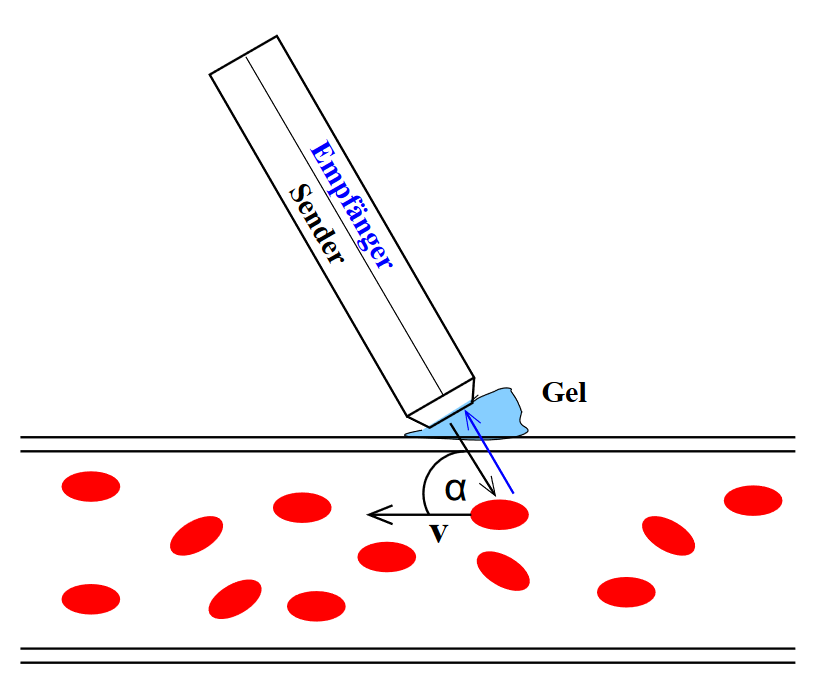
\includegraphics[width=\linewidth-70pt,height=0.3\textheight,keepaspectratio]{content/images/GesSkizze.png}
	\label{fig:GesSkizze}
\end{figure}

Bei der Sonographie wird mit Frequenzen im Ultraschallbereich gearbeitet. Diese sind für das Ohr des Menschen nicht wahrnehmbar und liegen zwischen ca. $\SI{20}{\kilo\hertz}$ und ca. $\SI{1}{\giga\hertz}$. Um diese Frequenzen zu erreichen und auch messen zu können werden der sogenannte reziproker piezoelektrischer Effekt und der piezoelektrischer Effekt genutzt.
Der reziproke piezoelektrische Effekt wird bei der Erzeugung der Schallwellen genutzt. Er besagt, dass sich ein piezoelektrischer Körper unter dem Einfluss eines elektrischen Feldes verformt, falls eine polare Achse in Richtung des Feldes zeigt. Durch die Verformung in einem periodische wechselnden Feld können somit Schallwellen vorgegebener Frequenz erzeugt werden, während bei der Resonanzfrequenz besonders große Amplituden erreicht werden können. Der piezoelektrische Effekt wird bei der Messung der Schallwellen genutzt. Er besagt, dass sich unter Verformung eines piezoelektrischer Körper ein elektrisches Feld aufbaut, welches in Form einer Spannung gemessen werden kann. Dadurch kann über die Verformung des Körpers durch die Schallwellen, diese wieder in elektrische Signale umgewandelt werden.